\title{Quadratic Forms}
\subtitle{\SubTitleName}
\institute[]{\Course}
\author{\Instructor}
\maketitle   
  



\frame{\frametitle{Topics and Objectives}
    \Emph{Topics} \\
    %\TopicStatement
    \begin{itemize}
    
        \item representing quadratic forms with symmetric matrices
        % \item Change of variables
        % \item Principle axes theorem
        % \item Classifying quadratic forms
    
    \end{itemize}
    
    \vspace{0.5cm}
    
    \Emph{Learning Objectives}\\
    
    %\LearningObjectiveStatement
    
    \begin{itemize}
    
        % \item characterize and classify quadratic forms using eigenvalues and eigenvectors
        \item express quadratic forms in the form $Q (\vec x ) =  \vec x ^{\, T} A \vec x$
        % \item Apply the principle axes theorem to express quadratic forms with no cross-product terms.
        
    \end{itemize}
    
    \vspace{0.25cm} 
    


} 





\begin{frame}{A Motivating Question}

    The equation $5x^2 + 4 xy + 8 y ^2 = 4$ represents an ellipse 
    \begin{center}
    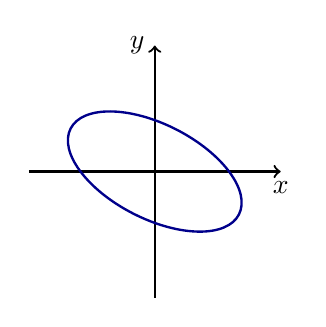
\begin{tikzpicture}[scale=0.4]
            \onslide<2->{ 
            \draw[->,thick]  (-4,0) -- (4,0)  node [below] {$x$}; 
            \draw[->,thick]  (0,-4) -- (0,4) node [left] {$y$}; 
            }
            \onslide<3->{
                \draw[rotate=63, DarkBlue, line width = 0.3mm] (0, 0) ellipse (1.5cm and 3cm);
            }
    \end{tikzpicture}
    \end{center} 
    \onslide<4->{An ellipse is an example of a \Emph{quadratic form}.} \onslide<5->{ If we can represent quadratic forms using a symmetric matrix, we can take advantage of the properties that symmetric matrices have to them.} \onslide<6->{How might we represent a quadratic form using a symmetric matrix? }
    
\end{frame}


\begin{frame}\frametitle{What are Quadratic Forms?}
    
    \begin{center}\begin{tikzpicture} \node [mybox](box){\begin{minipage}{0.90\textwidth}\vspace{2pt}
    A \Emph{quadratic form} is a function $ Q \;:\; \mathbb R ^{n} \to \mathbb R $, given by 
    \begin{equation*}
        Q (\vec x ) =  \vec x ^{\, T} A \vec x   = 
    \begin{pmatrix}
        x_1 & x _2 & \cdots & x_n 
    \end{pmatrix} \begin{pmatrix}
        a_ {11} & a _{12} & \cdots & a _{1n} 
        \\
        a _{12} & a _{22}  & \cdots & a _{2n} 
        \\ 
        \vdots &   \vdots & \ddots &   \vdots 
        \\
        a _{1n} & a _{2n} & \cdots & a _{nn}
    \end{pmatrix}
    \begin{pmatrix}
        x_1 \\ x _2\\ \vdots \\ x_n 
    \end{pmatrix}
    \end{equation*}
    Matrix $ A$ is $n \times n$ and symmetric.  
    \end{minipage}};
    \node[fancytitle, right=10pt] at (box.north west) {Definition};
    \end{tikzpicture}\end{center}
    
    In the above, $\vec x$ is a vector of variables. 

\end{frame}

\begin{frame} \frametitle{Quadratic Forms and Symmetric Matrices}
    Compute the quadratic form $Q =\vec x \, ^{T} A \vec x$, using  $\vec x = \begin{pmatrix}x\\y\end{pmatrix}$.
    \begin{align*}
    \text{(a)} \quad A = \begin{pmatrix} 4  & 0 \\ 0 & 3 \end{pmatrix} , \qquad
    \text{(b)} \quad A = \begin{pmatrix} 4  & 1 \\ 1 & -3 \end{pmatrix} 
\end{align*}

    \onslide<2->{
    \Emph{Solutions}}
    \begin{align*}
        \onslide<3->{\text{(a)} \quad Q &= \spalignmat{x y}\begin{pmatrix} 4  & 0 \\ 0 & 3 \end{pmatrix} \spalignmat{x;y} =\spalignmat{x y}\spalignmat{4x;3y} = 4x^2 +3y^2 }\\
        \onslide<4->{
        \text{(b)} \quad Q &= \spalignmat{x y}\begin{pmatrix} 4  & 1 \\ 1 & -3 \end{pmatrix} \spalignmat{x;y} =\spalignmat{x y}\spalignmat{4x+y;x-3y} = 4x^2 - 3y^2 +2xy
        }
    \end{align*}
    \onslide<5->{
    The $2xy$ term is a \Emph{cross-product} term because it contains both variables.}

\end{frame}

\begin{frame}{A Quadratic Form}

    Express
    \begin{equation*}
        Q = x^2 - 6 xy + 9 y ^2 
    \end{equation*}
    in the form $Q = \vec x^T A \vec x$, where $\vec x \in \mathbb R^2$ and $A=A^T$. 
    
    \vspace{12pt}
    
    \pause 
    \Emph{Solution}\\
    Placing coefficients of $x^2$ and $y^2$ on main diagonal, and dividing coefficient of $xy$ by 2, we obtain
    $$x^2 - 6 xy + 9 y ^2 = \begin{pmatrix} x & y \end{pmatrix} \spalignmat{1 -3;-3 9} \begin{pmatrix} x \\ y \end{pmatrix}
    $$
    We can verify this result by multiplying $\vec x \, ^T A \vec x$. 
\end{frame}


\begin{frame}\frametitle{Example: Quadratic Form in Three Variables}

     Write $Q$ in the form $\vec x^{T} A \vec x  $ for $\vec x \in \mathbb R^3$. 
     $$Q (\vec x) =  5 x_1 ^2 - x_2 ^2 + 3 x_3 ^2 +6 x_1 x_3 - 12 x_2 x_3$$
    
    \pause 
    \Emph{Solution}\\
    Note that we can write $Q$ as 
    $$Q =  5 x_1 ^2 - x_2 ^2 + 3 x_3 ^2 +6 x_1 x_3 - 12 x_2 x_3 + 0 x_1x_2$$
    Taking a similar approach to the previos exercise, we obtain
    $$Q = \begin{pmatrix} x_1 & x_2 & x_3 \end{pmatrix} \spalignmat{5 0 3;0 -1 -6;3 -6 3} \begin{pmatrix} x_1 \\ x_2 \\ x_3 \end{pmatrix}
    $$
    Again, we can verify this result by multiplying $\vec x \, ^T A \vec x$.     
\end{frame}




\begin{frame}\frametitle{Notes on Quadratic Forms}

    \begin{itemize}
        \item<1-> One of the reasons we are interested in quadratic forms relates to their use in describing linear transforms.
        \item<2-> Consider the transform $\vec x \to A\vec x$. The squared length of the vector $A\vec x$ is a quadratic form: 
    $$\lVert A \vec x \rVert^2 = (A\vec x) \cdot (A\vec x) = \vec x \, ^T A^TA \vec x$$
        \item<3-> Note that $A^TA$ is symmetric. 
        \item<4-> In other words, we can use symmetric matrices and their properties to, for example, characterize linear transforms.
    \end{itemize}
    
\end{frame}


\frame{\frametitle{Summary}

    \SummaryLine \vspace{4pt}
    \begin{itemize}\setlength{\itemsep}{8pt}

        \item the representation of quadratic forms with symmetric matrices

    \end{itemize}
    
    \vspace{6pt}
    \pause 
    We saw how we can express quadratic forms in the form $Q (\vec x ) =  \vec x ^{\, T} A \vec x$, for $\vec x \in \mathbb R^n$. 
    \pause
    
}